\section{Versuchsaufbau}
\label{sec:Versuchsaufbau}

Der Aufbau besteht aus einer Kammer mit einem Plattenkondensator und einer kleinen
Öffnung an der Oberseite. Die Oberseite dient dem Einfügen von zerstäubten Öltröpchen.
Die Plattenkondensatorplatten haben einen Abstand von $d = (7,6250 \pm 0,0051) \, \si{\milli\meter}$.\\
Um die Tröpchen gut sichbar zu machen, werden diese seitlich von einer Halogenlampe 
angestrahlt. Mit einem Thermowiderstand wird die Temperatur der Luft in der Kammer 
kontrolliert. Dieser Widerstand kann an einem Multimeter abgelesen werden. Die Spannung
zwischen den zwei Kondensatorplatten kann ebenfalls an einem Multimeter abgelesen werden.\\
Durch das Zerstäuben sind die meisten Öltröpchen geladen, manche allerdings nicht. Diese
können durch ein schwach radioaktives $\alpha$-Präparat ionisiert werden. Das Präparat kann
man mithilfe eines Schalters abschirmen oder "aktivieren".\\
Mithilfe eines Schalters kann die Polung der Kondensatorplatten verändert werden. Mit einer
Libelle kann überprüft und eingestellt werden, ob die Apparatur gerade steht. Mit einem
Mikroskop können die Tröpchen beobachtet werden.\\
Die Apparatur ist in der \autoref{Abb:Versuchsaufbau} zu sehen.

\begin{figure}[H]
    \centering
    
    \caption{Schematischer Aufbau der Versuchsappartatur zum Millikan-Öltröpchen-Versuch.\cite{sample}}
    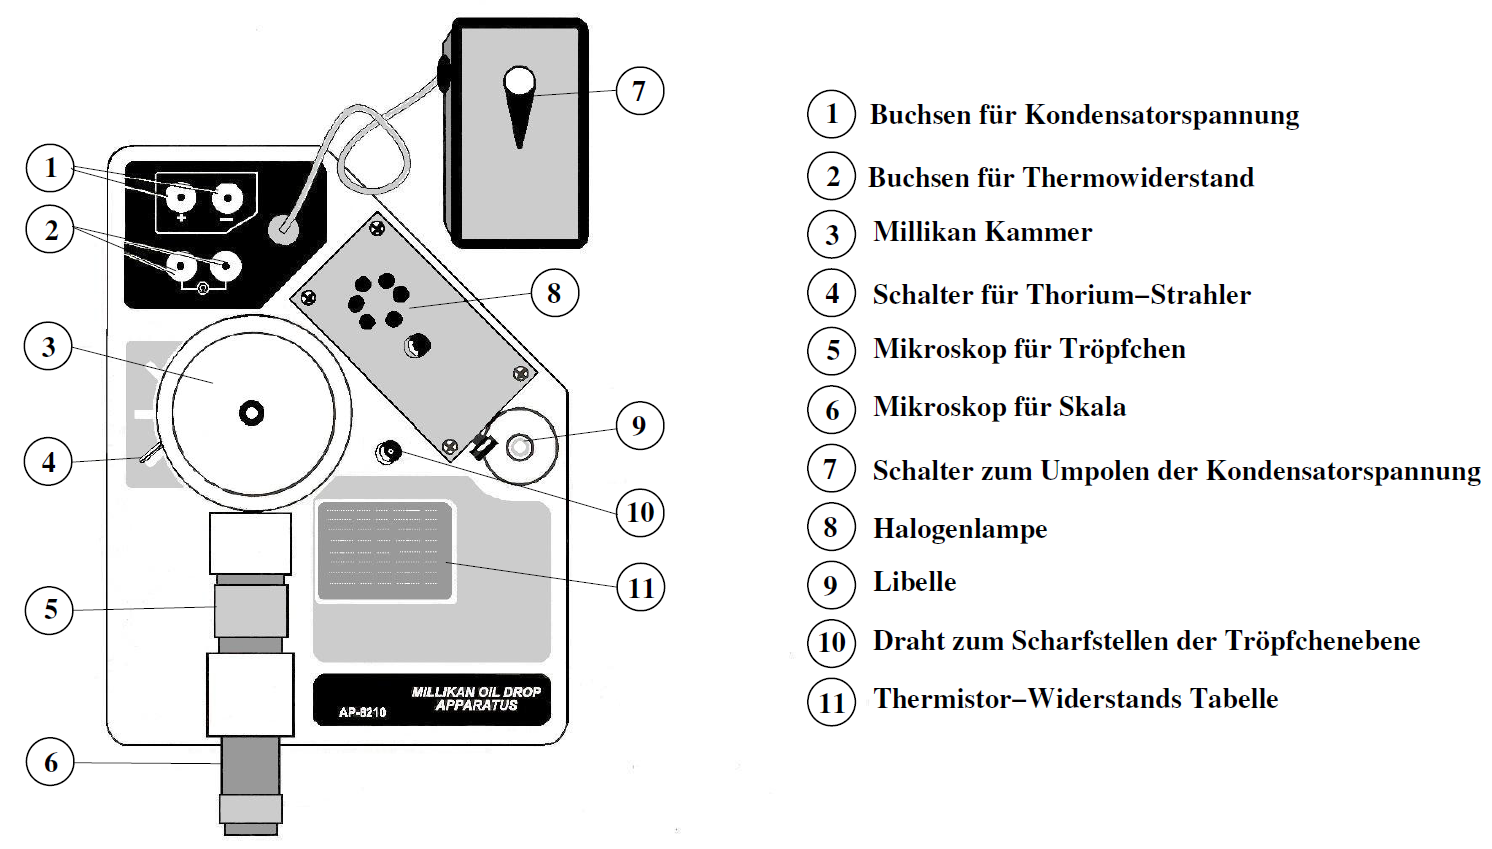
\includegraphics[width=\textwidth]{bilder/Versuchsaufbau.png}
    \label{Abb:Versuchsaufbau}
\end{figure}

\section{Durchführung}
\label{sec:Durchführung}

Zunächst wird überprüft ob die Apparatur waagerecht steht. Das erfolgt mithilfe der Libelle.
Dann werden die Platten geerdet und Öltröpchen in die Kammer gesprüht. Mithilfe des Mikroskops
wird während des Einsprühens überprüft, wie viele Tröpchen in die Kammer geraten. Bei zu vielen
Tröpchen gibt es zu viele Stöße zwischen diesen.\\
Bei fünf verschiedenen Spannung werden nun fünf verschiedene Tröpchen observiert. Es werden
jeweils die Zeiten notiert, die ein Tröpchen zum Aufsteigen einer festgelegten Strecke
und zum Absinken dieser Strecke benötigt. Die Aufstiegszeit und Abstiegszeit wird jeweils
drei Mal gemessen. Bei jedem Tröpchen wird vorher der Thermowiderstand gemessen.\\
Für die Spannungen werden 150 V, 170 V, 190 V, 210 V und 240 V verwendet. Durch das Umpolen
mithilfe des Schalters werden die Tröpchen immer in einer Aufwärtsbewegung beziehungsweise
Fallbewegung gebracht.\\
Durch gemessenen Werte für den Thermowiderstand kann man anhand der Tabelle in \autoref{fig:thermistor}
auf die Temperatur schließen.
